\documentclass{article}
\usepackage[utf8]{inputenc}

\usepackage{tgtermes}
\usepackage{fouriernc}
\usepackage[T1]{fontenc}
\usepackage[margin=3cm]{geometry}
\usepackage{listings}
\usepackage{hyperref}
\hypersetup{
    colorlinks=true,
    linkcolor=blue,
    filecolor=magenta,      
    urlcolor=cyan,
    pdftitle={Overleaf Example},
    pdfpagemode=FullScreen,
    }

\urlstyle{same}

\usepackage{amssymb}
\usepackage{amsmath}
\usepackage{graphics}

\usepackage{graphicx}

\usepackage{enumerate}
\usepackage{hyperref}


\newcommand{\N}{\mathbb{N}}
\newcommand{\Z}{\mathbb{Z}}
\newcommand{\Q}{\mathbb{Q}}
\newcommand{\R}{\mathbb{R}}
\linespread{1.5}

 
\title{Data viz project}
\author{Christine Søjberg, Heidi Lunde, Dennis Jønsson, Martin Slyngborg}
\date{Fall 2023}
  
\begin{document}
  
\maketitle

\section*{21/9}
- Sammenligne forskellige sygdomme. Vil fremkomst af en sygdom påvirke fremkomsten af en anden\\
- Gruppere på forskellige typer af sygdomme; eg. gun shot, violence etc. er en gruppe \\
\subsection*{Formål}
Beskrive udviklingen af dødsårsager i lande over tid

\subsection*{Data - i overordnede termer}
- Lande\\
- År\\
- Sygdomme\\
- BNP\\
- Befolkningstal\\
\subsection*{Ideas}
- \textbf{Barchart (udvikling)} (måske lidt det samme som stacked area??)(2)\\
- Scatter plot\\
- \textbf{Geospatial} (1)\\
- \textbf{Stacked column plot (multi)} (3)\\
- \textbf{Stacked area chart}(2) \\
- Matrix plot (facet)\\
- Boxplot/Violin plot\\

\subsection*{Final product layout}
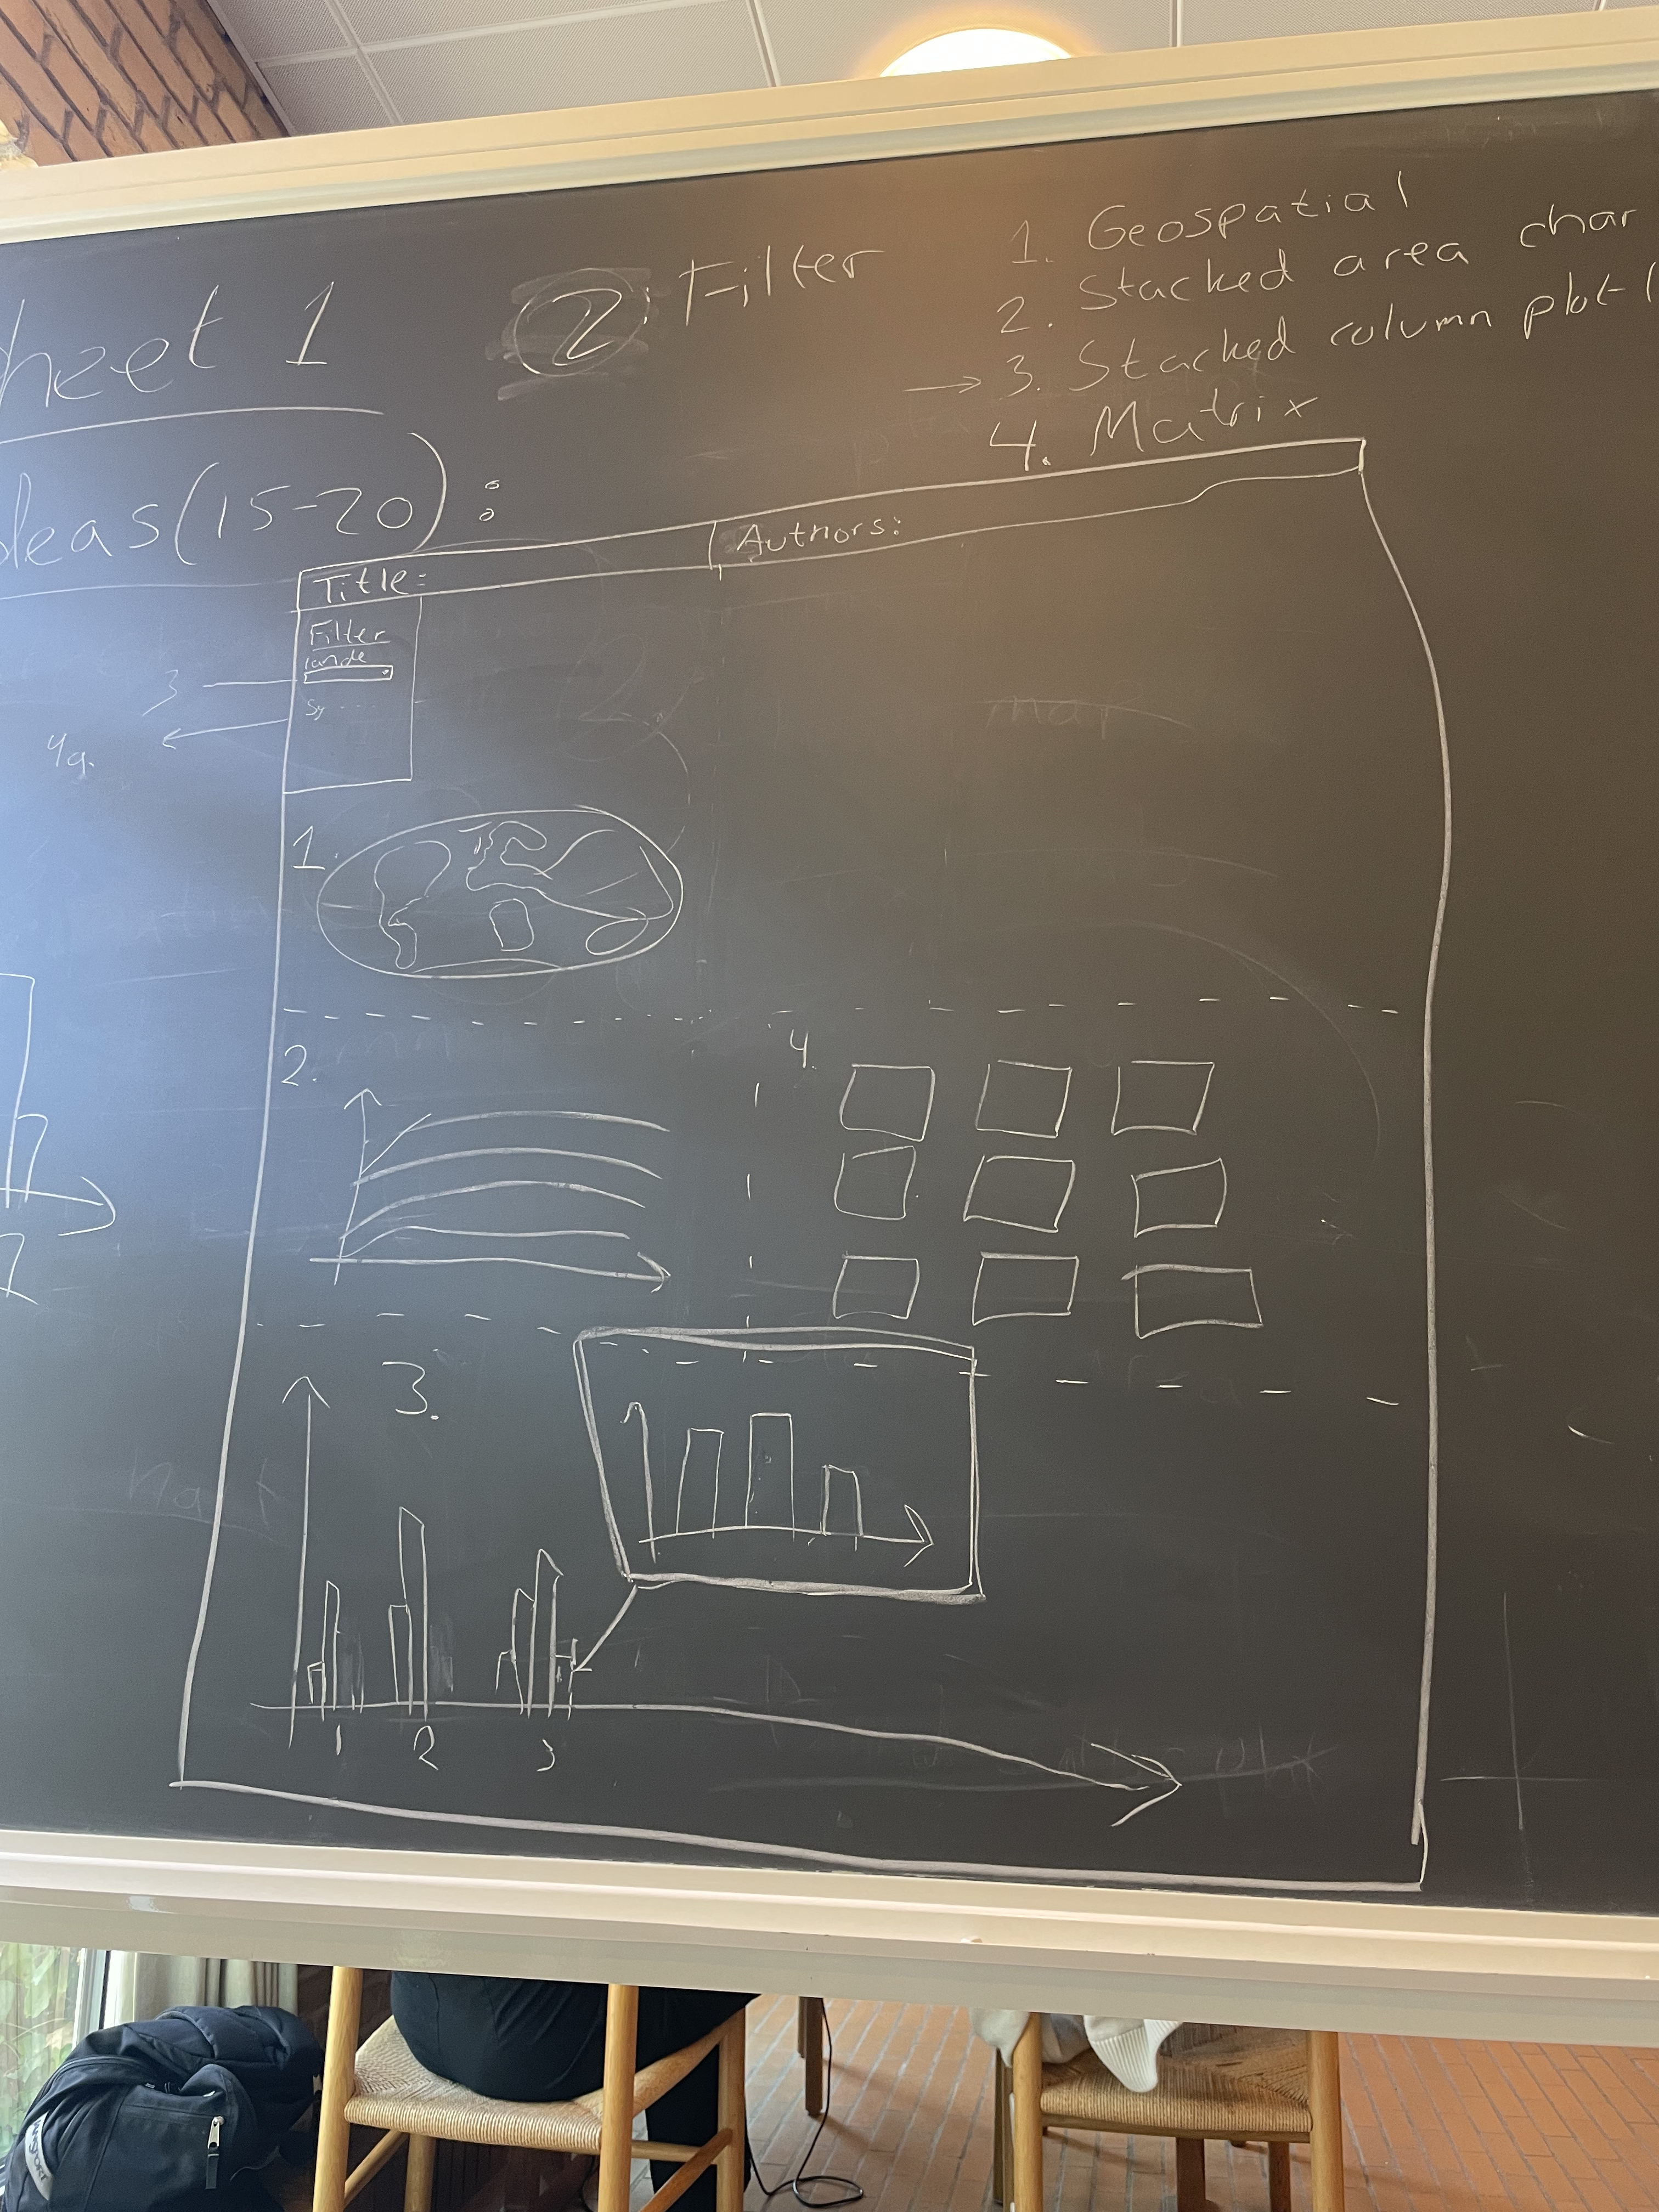
\includegraphics[scale = 0.1]{IMG_5366.png}

\newpage
\subsection*{Link to websites with python packages}
- \href{https://sites.northwestern.edu/researchcomputing/2022/02/03/what-is-the-best-interactive-plotting-package-in-python/}{northwestern.edu}\\

\section*{Calender}
\subsection*{26/9 - Uge 39}
- Prøve at få geomaps frem\\
- Teste i både VScode og jupyter\\
- Fokus: finde pakker og få dem til at virke med geospatial\\
\subsection*{Uge 40}
\subsection*{Uge 41}
\subsection*{Uge 42 - Ferie}
\subsection*{Uge 43}
\subsection*{Uge 44}
\subsection*{Uge 45}
\subsection*{Uge 46}
\subsection*{Uge 47}
\subsection*{Uge 48}
\end{document}
